\documentclass[a4paper, 12pt]{article}

% Packages
\usepackage[german]{babel}
\usepackage[top=4cm, bottom=2cm, left=4cm, right=2cm]{geometry}
\usepackage[utf8]{inputenc}
\usepackage[]{apacite}
\usepackage{fancyhdr}
\usepackage[multiple]{footmisc}
\usepackage{graphicx}
\usepackage{url}
\usepackage{pdfpages}
%\usepackage[hidelinks]{hyperref}

% Layout Einstellungen
%% Seitennummerierung oben mitte ohne durchgezogene Linie
\pagestyle{fancy}
\setlength{\headheight}{15pt}
\renewcommand\headrulewidth{0pt}
\chead{\thepage}
\lhead{}
\rhead{}
\lfoot{}
\cfoot{}
\rfoot{}
%% Zeilenabstand
\linespread{1.5}%\selectfont
%% Zeilenformatierung
%\fussy%
\sloppy
%% Abstand zwischen Absätzen
\setlength{\parskip}{2ex plus0.5ex minus0.5ex}
%% Keine Einrückung von Absätzen
\setlength{\parindent}{0em}
\bibliographystyle{apacite}

\begin{document}
	\includepdf{pdf/title.pdf}     
	\pagenumbering{Roman}
	\setcounter{page}{2}
	\tableofcontents
%	\listoffigures
	\clearpage
	\pagenumbering{arabic}
	\section{Einleitung}
Die wissenschaftliche Forschung wurde als wichtiger Einflussfaktor für die Entstehung neuer Technologien und Technologietrends in bedeutenden Studien nachgewiesen.\footnote{\citeNP<Vgl.>[S.~187]{Nelson1986}.}\footnote{\citeNP<Vgl.>[S.~11]{Mansfield1991}.}\footnote{\citeNP<Vgl.>[S.~599]{Tegarden2012}.}
Nach Jaffe wird diese Erkenntnis bereits durch die geographische Nähe von Zentren der Spitzentechnologie wie das "`Silicon Valley"' oder die "`Massachusetts Route 128"' zu führenden Universitäten gestützt.\footnote{Vgl. \citeNP{Jaffe1989}, S.~967f.} Nach einer Studie von Mansfield wären etwa 11~\% aller Produkte einer Auswahl aus sieben Fertigungsindustrien im Betrachtungszeitraum gar nicht oder nur mit erheblicher Zeitverzögerung entwickelt worden, wäre dem nicht eine entsprechende wissenschaftliche Forschung vorausgegangen.\footnote{\citeNP<Vgl.>[S.~2]{Mansfield1991}.}

Dennoch liegt die maßgebliche Entscheidung über den Einsatz und die Weiterentwicklung neuer Technologien vorwiegend in Händen von Unternehmern, Managern und sonstigen Entscheidungsträgern der praktizierenden Wirtschaft. Die wiederum richten ihre Entscheidungen unter Berücksichtigung einer Vielzahl von Faktoren an den Markt aus, um den Unternehmenserfolg zu steigern.\footnote{Vgl. \citeNP{Gruber2008}, S.~1652f.} Dabei greifen sie auch auf Informationsquellen von spezialisierten Unternehmen zurück, die mit Hilfe proprietärer Methoden Prognosen für Technologietrends in eigenen Publikationen herausgeben. Einer der einflussreichsten und bekanntesten Vertreter dessen ist der "`Gartner Hype Cycle"', den große Unternehmen bei strategischen Entscheidungen bezüglich neuer Technologien beratend hinzuziehen.\footnote{\citeNP<Vgl.>[S.~254]{Steinert2010}.}

Nach Beyer ist der Einfluss auf Technologietrends durch Wirtschaftsmedien höher als durch wissenschaftliche Artikel, da sie von Managern aufgrund des gewohnten Fachjargons sowie der Praxisrelevanz bevorzugt gelesen werden.\footnote{Vgl. \citeNP{Beyer1992}, S.~472.} Barley et al. fanden sogar heraus, dass sich gängige Begriffe der Wirtschaft in wissenschaftlicher Literatur verzögert manifestieren, folglich der Einfluss unidirektional von Unternehmern in Richtung Akademiker stattfindet.\footnote{Vgl. \citeNP{Barley1988}, S.~52.} Nach Spell hängt das allerdings eher damit zusammen, dass wissenschaftliche Artikel einem Peer-Review unterzogen werden, welcher Monate bis Jahre in Anspruch nehmen kann, bis sie in Fachartikeln erscheinen, als dass wissenschaftliche Forschungsschwerpunkte stets aus Wirtschaftsjournalen gespeist würden.\footnote{Vgl. \citeNP{Spell1999}, S.~345.}

\subsection{Problemstellung}
Somit findet eine gegenseitige Einflussnahme hinsichtlich der Prognose von Technologietrends zwischen Entscheidungsträgern der Wirtschaft und akademischen Forschern zweifelsohne statt. Gleichzeitig ist aufgrund teils unterschiedlicher Interessen beider Parteien eine Diskrepanz bei der Schwerpunktsetzung evident. 

Technologiethemen insbesondere in Informationstechnologien sind ständiger Ver\-änderung unterworfen\footnote{Vgl. \citeNP{Chang2009}, S.~107f.}, wodurch eine permanente Auseinandersetzung mit Trend\-themen für beide Seiten unumgänglich ist. Obwohl das "`Gartner Hype Cycle"' bei der Lösung dieser Herausforderung hohe Anerkennung in der Praxis genießt, bleibt es in der akademischen Forschung weitestgehend unberücksichtigt.\footnote{Vgl. \citeNP{OLeary2008}, S.~241.}\footnote{Vgl. \citeNP{Jarvenpaa2008}, S.~12.}

Folglich stellt sich die Frage, ob und in welchem Ausmaß sich prognostizierte Technologietrends aus der wirtschaftlichen Praxis in wissenschaftlichen Fachartikel widerspiegeln.

\subsection{Zielsetzung}
Das vorrangige Ziel der Arbeit ist es, über einen definierten Zeitraum Technologiethemen mit der höchsten medialen Präsenz in der Wirtschaft zu erfassen und die Verteilung dieser Themen in wissenschaftlichen Fachartikeln im Verhältnis gegenüberzustellen.

Dazu wird eine Datenbasis der Trendthemen aus dem "`Gartner Hype Cycle for Emerging Technologies"' für die jeweiligen Jahre des ausgewählten Zeitraumes entnommen. Anschließend werden diese Daten in mehreren Datenbanken für wissenschaftliche Fachartikel im vergleichbaren Zeitraum gesucht, um sie schließlich mit Hilfe quantitativer Methoden miteinander zu vergleichen.

Als Ergebnis der Analyse wird die Erkenntnis angestrebt, mögliche Diskrepanzen beim Verständnis für vielversprechende Trends festzustellen.

\subsection{Leitfragen}
Die einleitend genannte Feststellung, dass sich akademische Forschungsschwerpunkte im Bereich von neuen Technologien mit zeitlicher Verzögerung zur wirtschaftlichen Praxis etablieren, ist zum Ende des letzten Jahrhunderts gemacht worden. Der "`Gartner Hype Cycle"' ist etwa zur gleichen Zeit erstmalig im Jahre 1995 erschienen\footnote{Vgl. \citeNP{OLeary2008}, S.~241.} und findet folglich in diesen Artikeln keine Berücksichtigung.

Um die Aktualität dieser Erkenntnis zu eruieren, werden hieraus folgende Leitfragen abgeleitet:

\begin{description}
	\item[L1:] Wie ist das Verhältnis zwischen Technologien im Abschnitt "`Peak of Inflated Expectations"' und der Anzahl an wissenschaftlichen Publikationen im vergleichbaren Zeitraum?
\end{description}

\begin{description}
	\item[L2:] Ist eine erstmalig erschienene Technologie des "`Gartner Hype Cycle"' im Ab\-schnitt "`Peak of Inflated Expectations"' in wissen\-schaftlichen Ver\-öf\-fent\-lichungen als Trend wahrzunehmen?
\end{description}

\begin{description}
	\item[L3:] Wenn eine Technologie in einer späteren Ausgabe des "`Hype Cycle"' herausfällt, steigt die Anzahl wissenschaftlicher Artikel um eine gewisse Zeit weiter, bis sie stagniert bzw. abnimmt?
\end{description}

Durch die retrospektive Analyse vergangener Trendthemen können mit heutiger Betrachtung möglicherweise weitere Leitfragen hinsichtlich der Ursachen für Abweichungen aufgestellt werden, die als Grundlage für die weitere Forschung dienen können.

\subsection{Methodik}
Wegen der eingangs erwähnten Relevanz wird der "`Gartner Hype Cycle for Emerging Technologies"' als Stellvertreter für die wirtschaftliche Praxis bei der Bestimmung kommender Trendthemen angenommen. Dabei handelt es sich um die graphische Darstellung des üblicherweise zu beobachtenden Reifeprozesses einer neuen Technologie. In Abbildung \ref{fig:ghc_raw} ist der Rohaufbau einer solchen Graphik mit unter anderem dem Kurvenverlauf sowie den fünf Stufen bis zur Produktivität zu sehen. Der Abschnitt "`Peak of Inflated Expectations"' zeigt die Phase mit den größten, meist überzogenen Erwartungen an die Technologie, in der auch die Medienpräsenz am höchsten ist.\footnote{Vgl. \citeNP{Fenn2017}, S.~3f.} Deshalb werden die dort aufgeführten Technologien der neusten Ausgabe, welche einmal im Jahr erscheint, als Grundlage für den Trendvergleich verwendet.

Demgegenüber manifestieren sich Ergebnisse akademischer Forschung vorwiegend in wissenschaftlichen Fachartikeln, welche nach sog. \glqq Peer-Reviews\grqq \footnote{Prüfung durch Fachgenossen} in entsprechenden Zeitschriften veröffentlicht werden.\footnote{Vgl. \citeNP{Bucchi1996} S.~381.} Spezielle Web-Datenbanken bieten Möglichkeiten zur Suche und Anzeige solcher Artikel an.

Für die Suche der aus dem \glqq Gartner Hype Cycle \grqq ermittelten Technologien kommen zunächst einmal folgende Datenbanken für wissenschaftliche Literatur zum Einsatz:
\begin{enumerate}
	\item \url{http://ieeexplore.ieee.org/Xplore/home.jsp}
	\item \url{http://dl.acm.org}
	\item \url{http://ipscience.thomsonreuters.com/product/web-of-science}
\end{enumerate}

Falls die Menge an Ergebnissen nicht ausreichen sollte, wird folgende Datenbank ergänzt:

\url{http://www.sciencedirect.com}

Die Suchbegriffe werden gegebenenfalls erweitert oder taxonomisch zusammengefasst, falls ihre Verwendung in der wissenschaftlichen Literatur signifikant abweicht und dies somit erfordert.

\begin{figure}[h]
	\centering
	\caption{Struktur des \glqq Gartner Hype Cycle\grqq}
	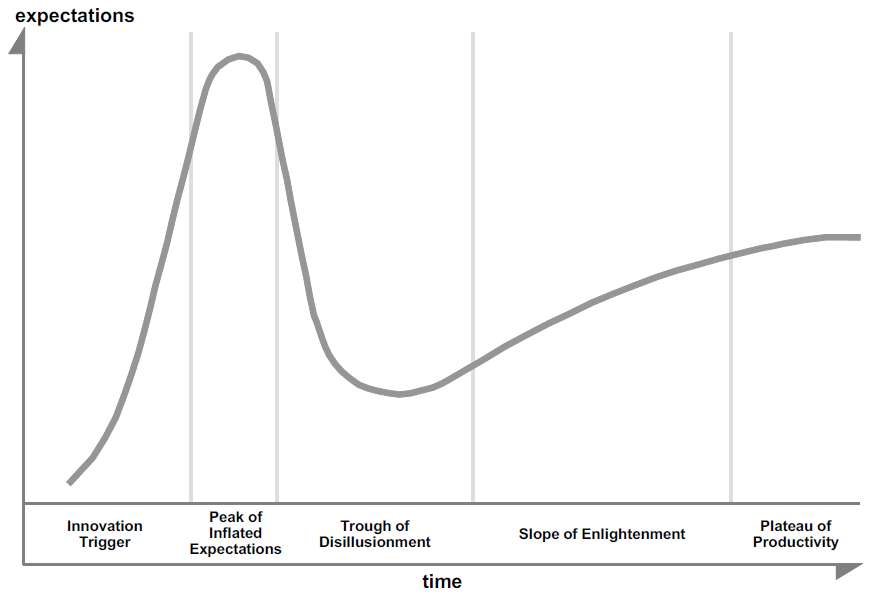
\includegraphics[width=0.9\linewidth]{img/ghc_raw}
	\caption*{\protect\fullciteNP<Quelle:>[S.~4]{Fenn2017}}
	\label{fig:ghc_raw}
\end{figure}

Anhand der Suchergebnisse wird jeder Technologie eine Matrix mit Suchmaschine, Jahr und Anzahl an Treffern zugeordnet. 

Der Betrachtungszeitraum für die Suche erstreckt sich über das Jahr des ersten Erscheinens einer der Technologien aus dem Abschnitt "`Peak of Inflated Expectations"' des "`Gartner Hype Cycle"' bis zum aktuellen Jahr. Das heißt, dass für die Ermittlung des Startjahres alle "`Hype Cycles"' der vergangenen Jahre in die Betrachtung einfließen, so lange mindestens eine der aktuellen Technologien im Abschnitt "`Peak of Inflated Expectations"' darin enthalten ist.

Alternativ kann das erstmalige Erscheinen einer Technologie im Abschnitt "`Innovation Trigger"' als Startzeitpunkt gewählt werden, sofern die Datenmenge im ersten Fall zu gering ausfällt.

Die ermittelte Verteilung der Mengen wird anschließend zunächst pro Suchmaschine und dann kumuliert betrachtet. Die dabei entstandene Kurve der Trefferanzahl über die Zeit wird dazu verwendet, die im Abschnitt "`Peak of Inflated Expectations"' erschienenen Technologien hinsichtlich des Trendverlaufes gegenüberzustellen.
	\renewcommand{\refname}{Literaturverzeichnis}
	\pagenumbering{roman}
	\lhead{}
	\linespread{1}
	\bibliography{lit}
\end{document}